\subsection{Concept Questions} % (fold)
\label{sub:array_concept_questions}

Read over the concepts in this chapter and answer the following questions:
\begin{enumerate}
  \item How is an array different to a standard variable?
  \item How do arrays make it easier to work with multiple values?
  \item Why is 0 the index of the first element in an array?
  \item How many bytes in memory would an array of 10 integers require?
  \item Draw a picture to show how the 10 integer values are stored in memory. Indicate how these values relate to the array.
  \item How can you access an element from an array?
  \item How can you copy the contents of one array into another array?
  \item Why should you pass an array to a parameter by reference, rather than by value?
  \item Can you perform an action on all elements of an array?
  \item How should you \emph{rethink} actions that needs to be performed on all elements in an array?
  \item How does the for loop work together with an array to perform an action on each element in an array?
  \item Why is a string an array? What values are stored in the elements of a string?
  \item Strings in C and Pascal have a single byte overhead. What is this overhead for? Why is it needed?
  \item Can you read/write past the end of an array (i.e. reading/writing to the 11th element when the array only contains 10 elements)? What can happen if you do this?
\end{enumerate}

\bigskip

\csection
{
\begin{enumerate}
  \item In C you need to pass an additional size parameter for any arrays passed in a function/procedure call. Explain why this is needed.
\end{enumerate}
}

\clearpage
% subsection concept_questions (end)

\subsection{Code Reading Questions} % (fold)
\label{sub:code_reading_questions_array}

Use what you have learnt to read and understand the following code samples.
\begin{enumerate}
  \item Read the C code in \lref{clst:all-below}, or the Pascal code in \lref{plst:all-below}, and answer the following questions:
  \begin{enumerate}
    \item What does the code do?
    \item What would be a good name for this function?
    \item Why is the array passed in using the const modifier?
    \item Will arrays be passed in by value or by reference when this function is called?
  \end{enumerate}
  \begin{figure}[h]
    \csection{\ccode{clst:all-below}{What does this C function do?}{topics/arrays/exercises/all-below.c}}
  \end{figure}
  \begin{figure}[h]
    \passection{\pascode{plst:all-below}{What does this Pascal function do?}{topics/arrays/exercises/AllBelow.pas}}
  \end{figure}
  
  \clearpage
  \item Read the C code in \lref{clst:contains}, or the Pascal code in \lref{plst:contains}, and answer the following questions:
  \begin{enumerate}
    \item What does the code do?
    \item What would be a good name for this function?
    \item What is returned by the function if it is passed ... 
    
    \begin{table}[h]
      \centering
      \begin{tabular}{|c|c|c|}
      \hline
       \textbf{data[]} & \textbf{sz} (C only)  & \textbf{val}  \\
       \hline 
       \{ 1, 2, 3, 4 \} & 4 & 3 \\
       \hline
       \{ 7, 12, 20, 51, -6 \} & 5 & 10 \\
       \hline
       \{ 2, 7, 1 \} & 3 & 1 \\
       \hline
       \{ -1, -2, -3, -4 \} & 4 & -3 \\
       \hline
       \{ 6, 12, 18, 24, 30 \} & 5 & 22 \\
       \hline
      \end{tabular}
    \end{table}
    
      \end{enumerate}
  \begin{figure}[h]
    \csection{\ccode{clst:contains}{What does this C function do?}{topics/arrays/exercises/contains.c}}
  \end{figure}
  \begin{figure}[h]
    \passection{\pascode{plst:contains}{What does this Pascal function do?}{topics/arrays/exercises/Contains.pas}}
  \end{figure}
  
  \clearpage
  \item The following code is designed to find the median (middle value) of a array of numbers, but does it work? Read the C code in \lref{clst:median}, or the Pascal code in \lref{plst:median}, and answer the following questions:
  \begin{enumerate}
    \item Assume that data := [1,2,3,4,5,6,7,8], execute this code by hand and show the steps involved. Explain any shortcuts you take.
    \item What value is returned when the function ends?
    \item You should have noticed that there is a bug in this program. How can it be fixed?
    \item What does this program assume about the data in the array?
    \item Can you think of a simpler solution? Explain your solution.
  \end{enumerate}
  \begin{figure}[h]
    \csection{\ccode{clst:median}{A median function written using C}{topics/arrays/exercises/median.c}}
  \end{figure}
  \begin{figure}[h]
    \passection{\pascode{plst:median}{A median function written using Pascal}{topics/arrays/exercises/Median.pas}}
  \end{figure}

  \clearpage
  \item Read the C code in \lref{clst:insert_at}, or the Pascal code in \lref{plst:insert_at}, and answer the following questions:
  \begin{enumerate}
    \item This procedure alters the array passed to it. Hand execute the procedure for the values shown in the following table. Record your workings as well as the final answer.
    \item What does the code do?
    \item What would be a good name for this procedure?
    \item What would be good names for \texttt{param3} and \texttt{param4}?
    
    \begin{table}[h]
      \centering
      \begin{tabular}{|c|c|c|c|}
      \hline
       \textbf{data[]} & \textbf{sz} (C only)  & \textbf{param3} & \textbf{param4}  \\
       \hline 
       \{ 1, 2, 3, 4 \} & 4 & 2 & 10 \\
       \hline
       \{ 8, 10, 11 \} & 3 & 1 & 9 \\
       \hline
       \{ -1, -2, -3, -4 \} & 4 & 0 & 0 \\
       \hline
       \{ 42, 42 \} & 2 & 1 & 73 \\
       \hline
      \end{tabular}
    \end{table}
    
      \end{enumerate}
  \begin{figure}[h]
    \csection{\ccode{clst:insert_at}{What does this C function do?}{topics/arrays/exercises/insert-at.c}}
  \end{figure}
  \begin{figure}[h]
    \passection{\pascode{plst:insert_at}{What does this Pascal function do?}{topics/arrays/exercises/InsertAt.pas}}
  \end{figure}

\end{enumerate}
% subsection code_reading_questions (end)
\clearpage
\subsection{Code Writing Questions: Applying what you have learnt} % (fold)
\label{sub:code_writing_questions_applying_what_you_have_learnt_array}

Apply what you have learnt to the following tasks:
\begin{enumerate}
  \item Create a program that reads in the user's name and then outputs the message `Hello ' and the users name. For example, if the user enters the name `Fred' then the program outputs the message `Hello Fred!' to the Terminal. See \tref{tbl:hello-user}.
  
  \begin{table}[h]
  \centering
  \begin{tabular}{l|p{12cm}}
    \hline
    \multicolumn{2}{c}{\textbf{Program Description}} \\
    \hline
    \textbf{Name} & \emph{Hello User} \\
    \\
    \textbf{Description} & Asks the user to enter their name, and then outputs `Hello ' and their name to the Terminal. \\
    \hline
  \end{tabular}
  \caption{Description of the \emph{Hello User} program.}
  \label{tbl:hello-user}
  \end{table}
  
  \item Create a program that reads in the user's name and then determines if the name is a \emph{silly name}. For example, if the user enters the name `Fred' the program could output, `Fred is an awesome name!', but if the user enters any other name they get a message like `Andrew is a silly name!'. Customise the message for your friends and tutor. See \tref{tbl:silly_name}.

  \begin{table}[h]
  \centering
  \begin{tabular}{l|p{12cm}}
    \hline
    \multicolumn{2}{c}{\textbf{Program Description}} \\
    \hline
    \textbf{Name} & \emph{Silly Name Test} \\
    \\
    \textbf{Description} & Asks the user to enter their name, and then outputs a message based on the name entered. \\
    \hline
  \end{tabular}
  \caption{Description of the \emph{Silly Name} program.}
  \label{tbl:silly_name}
  \end{table}
  
  \clearpage
  \item Complete the implementation of the Statistics Calculator. Then add the following additional functionality:
  \begin{enumerate}
      \item Add a \textbf{Print All} procedure to print all of the values stored in the array to the Terminal.
      \begin{figure}[h]
        \csection{\csnipet{void print_all(const int data[], int sz)}\ldots}
        \passection{\passnipet{procedure PrintAll(const data: array of Integer);}\ldots}
      \end{figure}

      \item Add a \textbf{Frequency} function that calculates the frequency of a value in the array.
\begin{figure}[h]
  \csection{\csnipet{int frequency(const int data[], int sz, int n)}\ldots}
  \passection{\passnipet{function Frequency(const data: array of Integer; n: Integer): Integer;}\ldots}
\end{figure}

      \item Add a \textbf{Standard Deviation} function.
      \begin{figure}[h]
        \csection{\csnipet{int stddev(const int data[], int sz)}\ldots}
        \passection{\passnipet{function Stddev(const data: array of Integer): Integer;}\ldots}
      \end{figure}

      \item Add a \textbf{Minimum} function.
      \begin{figure}[h]
        \csection{\csnipet{int min(const int data[], int sz)}\ldots}
        \passection{\passnipet{function Min(const data: array of Integer): Integer;}\ldots}
      \end{figure}
  \end{enumerate}
  \clearpage
  \item Implement the Bubble Game from \sref{sub:bubble_game_start_} \nameref{sub:bubble_game_start_}. You will need to do the following:
  \begin{enumerate}
    \item Download the appropriate SwinGame template.
    \item Extract the template into a folder called `Bubbles'
    \item Find a picture of a bubble that is about 30 pixels wide and high.
    \item Place the bubble image in the \texttt{Resources/images} folder in your SwinGame project.
    \item Implement the code from \sref{sub:bubble_game_start_}.
    \item Run the game and you should something similar to \fref{fig:bubble_game}.
  \end{enumerate}
  
  \begin{figure}[h]
     \centering
     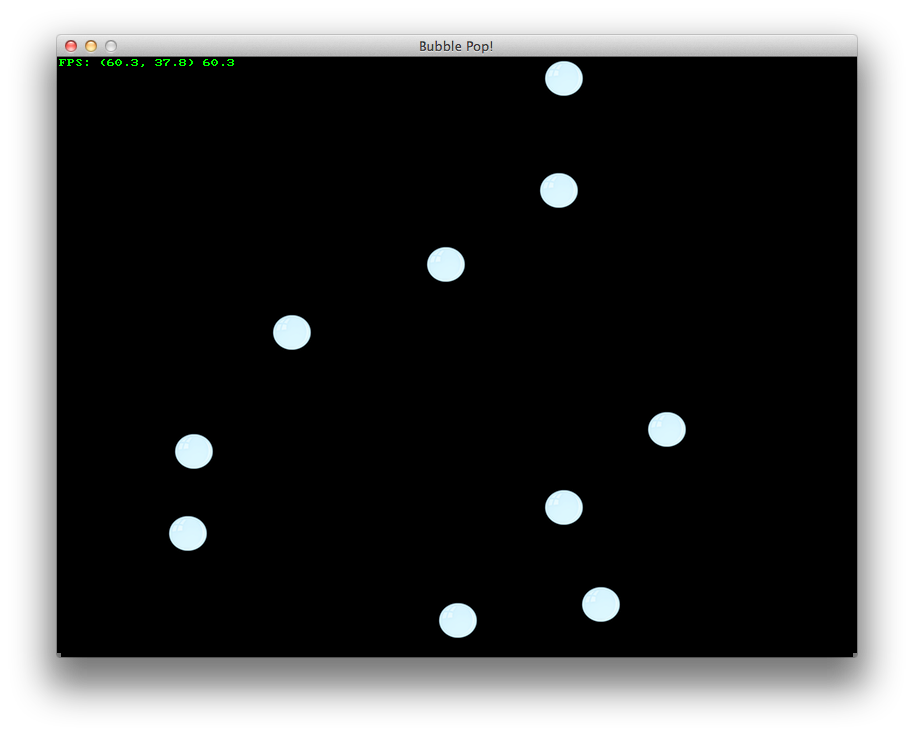
\includegraphics[width=0.6\textwidth]{./topics/arrays/exercises/BubblesGame.png} 
     \caption{The start of a bubble game}
     \label{fig:bubble_game}
  \end{figure}
  
  \item Try extending the game in one or more of the following ways:
  
 \begin{enumerate}
  \item Play a sound effect when the bubbles appear.
  \item Add a background image.
  \item Check if the user has clicked the bubble. If they have, play a pop sound effect and place the bubble.
  \item Add a score, and give points for the number of bubbles popped.
  \item Try changing the game dynamics... add gravity and have the bubbles pop when they hit the ground, ending the game. Start new bubbles at the top of the screen.
  \item \ldots
 \end{enumerate}
  
\end{enumerate}
% subsection code_writing_questions_applying_what_you_have_learnt (end)

\clearpage
\subsection{Extension Questions} % (fold)
\label{sub:extension_questions_array}

If you want to further your knowledge in this area you can try to answer the following questions. The answers to these questions will require you to think harder, and possibly look at other sources of information.
\begin{enumerate}
  \item Write the code to sort the values in your statistic calculator.
  \item Write a function that calculates the \textbf{Mode}, the most frequent value.
  \item Get your bubbles to bounce off each other. Hint: have a look at SwinGame physics \textbf{Collide Circles} procedure.

% subsection extension_questions (end)
  
  
  
\end{enumerate}